% Template for PLoS
% Version 3.5 March 2018
%
% % % % % % % % % % % % % % % % % % % % % %
%
% -- IMPORTANT NOTE
%
% This template contains comments intended 
% to minimize problems and delays during our production 
% process. Please follow the template instructions
% whenever possible.
%
% % % % % % % % % % % % % % % % % % % % % % % 
%
% Once your paper is accepted for publication, 
% PLEASE REMOVE ALL TRACKED CHANGES in this file 
% and leave only the final text of your manuscript. 
% PLOS recommends the use of latexdiff to track changes during review, as this will help to maintain a clean tex file.
% Visit https://www.ctan.org/pkg/latexdiff?lang=en for info or contact us at latex@plos.org.
%
%
% There are no restrictions on package use within the LaTeX files except that 
% no packages listed in the template may be deleted.
%
% Please do not include colors or graphics in the text.
%
% The manuscript LaTeX source should be contained within a single file (do not use \input, \externaldocument, or similar commands).
%
% % % % % % % % % % % % % % % % % % % % % % %
%
% -- FIGURES AND TABLES
%
% Please include tables/figure captions directly after the paragraph where they are first cited in the text.
%
% DO NOT INCLUDE GRAPHICS IN YOUR MANUSCRIPT
% - Figures should be uploaded separately from your manuscript file. 
% - Figures generated using LaTeX should be extracted and removed from the PDF before submission. 
% - Figures containing multiple panels/subfigures must be combined into one image file before submission.
% For figure citations, please use "Fig" instead of "Figure".
% See http://journals.plos.org/plosone/s/figures for PLOS figure guidelines.
%
% Tables should be cell-based and may not contain:
% - spacing/line breaks within cells to alter layout or alignment
% - do not nest tabular environments (no tabular environments within tabular environments)
% - no graphics or colored text (cell background color/shading OK)
% See http://journals.plos.org/plosone/s/tables for table guidelines.
%
% For tables that exceed the width of the text column, use the adjustwidth environment as illustrated in the example table in text below.
%
% % % % % % % % % % % % % % % % % % % % % % % %
%
% -- EQUATIONS, MATH SYMBOLS, SUBSCRIPTS, AND SUPERSCRIPTS
%
% IMPORTANT
% Below are a few tips to help format your equations and other special characters according to our specifications. For more tips to help reduce the possibility of formatting errors during conversion, please see our LaTeX guidelines at http://journals.plos.org/plosone/s/latex
%
% For inline equations, please be sure to include all portions of an equation in the math environment.  For example, x$^2$ is incorrect; this should be formatted as $x^2$ (or $\mathrm{x}^2$ if the romanized font is desired).
%
% Do not include text that is not math in the math environment. For example, CO2 should be written as CO\textsubscript{2} instead of CO$_2$.
%
% Please add line breaks to long display equations when possible in order to fit size of the column. 
%
% For inline equations, please do not include punctuation (commas, etc) within the math environment unless this is part of the equation.
%
% When adding superscript or subscripts outside of brackets/braces, please group using {}.  For example, change "[U(D,E,\gamma)]^2" to "{[U(D,E,\gamma)]}^2". 
%
% Do not use \cal for caligraphic font.  Instead, use \mathcal{}
%
% % % % % % % % % % % % % % % % % % % % % % % % 
%
% Please contact latex@plos.org with any questions.
%
% % % % % % % % % % % % % % % % % % % % % % % %

\documentclass[10pt,letterpaper]{article}
\usepackage[top=0.85in,left=2.75in,footskip=0.75in]{geometry}

% amsmath and amssymb packages, useful for mathematical formulas and symbols
\usepackage{amsmath,amssymb}

% Use adjustwidth environment to exceed column width (see example table in text)
\usepackage{changepage}

% Use Unicode characters when possible
\usepackage[utf8x]{inputenc}

% textcomp package and marvosym package for additional characters
\usepackage{textcomp,marvosym}

% cite package, to clean up citations in the main text. Do not remove.
\usepackage{cite}

% Use nameref to cite supporting information files (see Supporting Information section for more info)
\usepackage{nameref,hyperref}
\usepackage[romanian]{babel}
\usepackage{combelow}

% line numbers
\usepackage[right]{lineno}

% ligatures disabled
\usepackage{microtype}
\DisableLigatures[f]{encoding = *, family = * }

% color can be used to apply background shading to table cells only
\usepackage[table]{xcolor}

% array package and thick rules for tables
\usepackage{array}
\usepackage{soul}
% create "+" rule type for thick vertical lines
\newcolumntype{+}{!{\vrule width 2pt}}

% create \thickcline for thick horizontal lines of variable length
\newlength\savedwidth
\newcommand\thickcline[1]{%
  \noalign{\global\savedwidth\arrayrulewidth\global\arrayrulewidth 2pt}%
  \cline{#1}%
  \noalign{\vskip\arrayrulewidth}%
  \noalign{\global\arrayrulewidth\savedwidth}%
}

% \thickhline command for thick horizontal lines that span the table
\newcommand\thickhline{\noalign{\global\savedwidth\arrayrulewidth\global\arrayrulewidth 2pt}%
\hline
\noalign{\global\arrayrulewidth\savedwidth}}


% Remove comment for double spacing
%\usepackage{setspace} 
%\doublespacing

% Text layout
\raggedright
\setlength{\parindent}{0.5cm}
\textwidth 5.25in 
\textheight 8.75in

% Bold the 'Figure #' in the caption and separate it from the title/caption with a period
% Captions will be left justified
\usepackage[aboveskip=1pt,labelfont=bf,labelsep=period,justification=raggedright,singlelinecheck=off]{caption}
\renewcommand{\figurename}{Fig}

% Use the PLoS provided BiBTeX style
\bibliographystyle{plos2015}

% Remove brackets from numbering in List of References
\makeatletter
\renewcommand{\@biblabel}[1]{\quad#1.}
\makeatother



% Header and Footer with logo
\usepackage{lastpage,fancyhdr,graphicx}
\usepackage{epstopdf}
%\pagestyle{myheadings}
\pagestyle{fancy}
\fancyhf{}
%\setlength{\headheight}{27.023pt}
%\lhead{\includegraphics[width=2.0in]{PLOS-submission.eps}}
\rfoot{\thepage/\pageref{LastPage}}
\renewcommand{\headrulewidth}{0pt}
\renewcommand{\footrule}{\hrule height 2pt \vspace{2mm}}
\fancyheadoffset[L]{2.25in}
\fancyfootoffset[L]{2.25in}
\lfoot{\today}

%% Include all macros below

\newcommand{\lorem}{{\bf LOREM}}
\newcommand{\ipsum}{{\bf IPSUM}}

%% END MACROS SECTION


\begin{document}
\vspace*{0.2in}

% Title must be 250 characters or less.
\begin{flushleft}
{\Large
\textbf\newline{The Impact of COVID-19 on Fertility behaviour and Intentions in a middle income country} % Please use "sentence case" for title and headings (capitalize only the first word in a title (or heading), the first word in a subtitle (or subheading), and any proper nouns).
}
\newline
% Insert author names, affiliations and corresponding author email (do not include titles, positions, or degrees).
\\
Tom Emery\textsuperscript{1*},
Judith Koops\textsuperscript{2}\textsuperscript{3},
\\
\bigskip
\textbf{1} Department of Public Administration, Erasmus University Rotterdam, Rotterdam, Netherlands
\\
\textbf{2} Netherlands Interdisciplinary Demographic Institute, Den Haag, Netherlands
\\
\textbf{3} University of Groningen, Groningen, Netherlands
\\
\bigskip

% Insert additional author notes using the symbols described below. Insert symbol callouts after author names as necessary.
% 
% Remove or comment out the author notes below if they aren't used.


% Use the asterisk to denote corresponding authorship and provide email address in note below.
* tom@odissei-data.nl

\end{flushleft}
% Please keep the abstract below 300 words
\section*{Abstract}
The COVID Pandemic may affect fertility behaviour and intentions in many ways. Restrictions on service provision reduce access to family planning services and increase fertility in the short term. By contrast, the economic uncertainty brought about by the pandemic and its impact on mental health and well-being may reduce fertility. These various pathways have been explored in the context of high income countries such as the United States and Western Europe, but little is known about middle income countries. In this paper we asses the impact of the COVID pandemic on fertility intentions and behaviour in the Republic of Moldova, a middle income country in Eastern Europe, using the Generations and Gender Survey. This survey was conducted partially before and partially after the onset of the pandemic, allowing for detailed comparisons of individual circumstances. The results indicate that the pandemic reduced the used of intrauterine devices, and increased the use of condoms, but with no overall decrease in contraceptive use. Conversely individuals interviewed after the onset of the pandemic were 41\% less likely to be trying to conceive, although medium term fertility intentions were unchanged. Indicators therefore suggest that in the medium term fertility intentions may not be affected by the pandemic but \hl{restricted access to contraception and a decrease in short-term fertility intentions may increase unintended pregnancies, leading to a change in who has children and when}.

\linenumbers

% Use "Eq" instead of "Equation" for equation citations.
\section*{Introduction}
It is expected that the COVID-19 pandemic will influence fertility levels \cite{lappegaard2020covid}. Similar to previous crises – like the 2008 economic crisis - economic uncertainty can reduce the intention to have a child and therefore depress fertility behaviour. However, there is also something unique about the current crisis, namely, the pandemic's possible impact on access to family planning. The most effective and common way to reduce fertility is with the use of contraceptives. However, due to the current health-crisis, access to family planning services may actually be reduced in some contexts. In addition, the COVID-19 pandemic is different because it restricts the movement of people, people are at home more, and this may influence family relations and sexual activity  \cite{settersten2020understanding}. Tension between intentions on the one hand and actual behaviour on the other makes it unclear how the pandemic will affect the overall fertility level.

Most of the existing research on the impact of the pandemic on fertility behaviour has been concentrated on developed economies \cite{luppi2020impact}. Aassve et al. (2020) argue that the impact of the pandemic on fertility will largely be shaped by the socio-economic context of individuals. They argue that in high income countries, damage to work-life balance and the access to assisted reproductive technology will negatively affect fertility. This will be amplified by the increase in economic uncertainty, which evidence from the great recession of 2008 suggests will depress fertility levels. By contrast rural areas of low-income countries could observe an increase in fertility as access to family planning is curtailed and general development hampered or even declined\cite{aassve2020covid}.

They see greater uncertainty about the impact on fertility in middle income countries and particularly urban areas within them. In such places, Aassve et al. (2020) argue that it is unclear if reduced access to family planning would lead to an increase in fertility and whether this would offset any decrease in fertility brought about by the uncertain economic outlook. The puzzle presented is a complex one with multiple influences on the fertility intention and behaviour of individuals. Attempts have been made to conceptualize this and produce more precise workable hypotheses but these again focus on high income countries \cite{voicu2020fertility}. Whilst fertility data for 2020 will soon reveal the short-term impact of the pandemic on fertility, the aim here is to examine the role played by these competing causal pathways in shaping fertility behaviour at the individual level in a middle-income country such as the Republic of Moldova. In middle income countries it should also be noted that the impacts of the pandemic are likely to affect the population for longer given that vaccine role out is expected to be far slower in middle income countries than in high income countries.

\section*{Existing Research} \label{sec:existing}

\subsection*{Fertility intentions}

Research on the impact of the pandemic on fertility behaviour has been largely concentrated on high income countries, predominantly in Western Europe and North America. The evidence here has suggested a fall in fertility intentions in line with the hypothesis put forward by Aassve et al. (2020). Luppi, Arpino and Rosina (2020) demonstrated that fertility intentions had fallen in Spain, France, Italy, Germany and the UK but that this manifested itself differently in each context. In Italy, falls in fertility intentions were amongst the highly educated under 30’s whereas in Germany the patterns were geo-spatially concentrated in areas with the highest infection rates.

Research in Shanghai has demonstrated that fertility intentions amongst couples remain unaffected by the pandemic, especially if the couple themselves have faith in government and public health measures \cite{zhu2020fertility}. This is the only research to date that we were able to identify that wasn't focused on a high income, western society. They also noted that those who intended to defer pregnancy plans were particularly worried about the impact of the virus itself on the health of the mother and fetus.

Wilde (2020) used data on google search terms to estimate that births would fall by 15\% year on year by November 2020, reflecting a change in search term trends related to pregnancy and contraception \cite{wilde2020covid}. They also noted that the fall was expected to be even higher amongst low income households and those from minority groups. This observation is consistent with understanding that economic uncertainties effect on fertility behaviour will be greatest amongst those with the fewest resources. However, the effect is very large and would represent a fall in fertility that is several times larger than that observed with the onset of the great depression in 2008.

\subsection*{Sexual and Reproductive Health during the COVID-19 Pandemic}

COVID-19 and the associated social restrictions have raised concerns that access to family planning services could be restricted with significant consequences for family planning. The United Nations Population Division has suggested that the pandemic could result in 60 million fewer users of contraceptive methods worldwide \cite{dasgupta2020impact}. The impact of the pandemic is expected to be particularly acute in low and middle income countries. Projected declines are expected to be largest for injectables (-20\%), condoms (-10\%) and the pill (-10\%). The condom and the pill are pervasive in Eastern Europe and therefore the impact in this region could be particularly strong \cite{eeckhaut2014using}. Furthermore, it is expected that rural populations access to family planning services will be disproportionately affected during the pandemic as supply lines and services are more thinly distributed \cite{dasgupta2020impact}. It should be expected that contraceptive methods that require medical consultations will have particularly noticeable falls where as methods that can be used independently will be less affected..

Despite this there is currently little empirical data on the access to sexual and reproductive health services during the pandemic in low and middle income countries. The implicit assumption appears to be that access to family services in high income countries would be unaffected by the pandemic and associated restrictions on movement and businesses \cite{aassve2020covid}\cite{luppi2020impact}. The rationale for this belief is somewhat understandable as some forms of contraception are readily available. However, during the lockdown the office hours of doctors and various clinics were reduced, and services altered. \cite{lindberg2020early} showed that around 28\% of childbearing age in the United States worried about their access to sexual and reproductive health care due to the pandemic and 39\% saying they had delayed or cancelled such care services due to the pandemic. These concerns and limitations on access are greater amongst marginalized or vulnerable populations.

In addition to contraceptive use, a lockdown may lead to an increase in sexual activity \cite{matchan2020americans}. However, several surveys conducted during the pandemic have shown this to not be the case and that instead sexual activity appears to have declined \cite{jacob2020covid}. In addition to access to family planning services, there is also the risk that the disease itself may affect fertility levels. There is tentative evidence that the disease disproportionately effects male gonads and there is a potential risk of male sterility, although evidence is as of yet inconclusive \cite{jirge2020resuming}. 

\subsection*{The progression of the pandemic in the Republic of Moldova}

The aim of this paper is to examine the impact of the COVID pandemic on fertility in a middle income country. However, the analysis is limited to the Republic of Moldova which has several characteristics which make it atypical for middle income countries. The World Bank defines a middle income country as one in which GNP per capita is between \$4,046 and \$12,535. As of 2019, the Republic of Moldova is at the bottom end of this range at \$4,320. Most of these countries also  lie in Latin America, Asia and Africa, however the Republic of Moldova is a middle income country that borders the European Union and Ukraine. 

The Republic of Moldova also has specific features which are of relevance to the pandemic's impact. Due to the Republic of Moldova's proximity to countries with significantly higher income levels and extensive free-trade and association agreements with those countries the degree of out-migration and seasonal work migration is exceptionally large in the Republic of Moldova. Estimates by the UNFPA suggest that around 9.9\% of the working age population is abroad for work \cite{prodan2016impact})\footnote{population and migration estimates are currently under extensive revision. At the time of writing these figures were yet to be published but it is anticipated that the total population will be substantially lower}. This also means that remittances make up almost 12.5\% of Gross Domestic Product \cite{ito2017remittances}. Such extensive migration has in itself been shown to be disruptive to fertility intentions and their realization. In addition, the Republic of Moldova already \hl{had a low total fertility rate of around 1.27 in 2019 and it has been at this level since the turn of the century}. Due to extensive out migration and low fertility, the Republic of Moldova is a rapidly ageing society and its demographic resilience is a key policy concern for the Moldovan Government and especially regarding the impact of COVID-19 on wider socio-economic development. 

The progression of the pandemic in the Republic of Moldova was similar to that of many countries in Eastern Europe with low and moderate rates of infection relative to Western Europe in the early phase of the pandemic through March and April. However, there was a steady rise in cases through the summer and autumn months. The spread of the virus through the country has not been even. Anenii Noi, B\v{a}lți, Edine\cb{t} and Ialoveni had the highest \hl{cumulative number of cases per thousand} in the country peaking at around 35-40, with the capital Chișinău recording a rate of 83 (see figure~\ref{fig:map}). Rural areas had much lower case rates than these urban centres. 

\begin{figure}
\centering
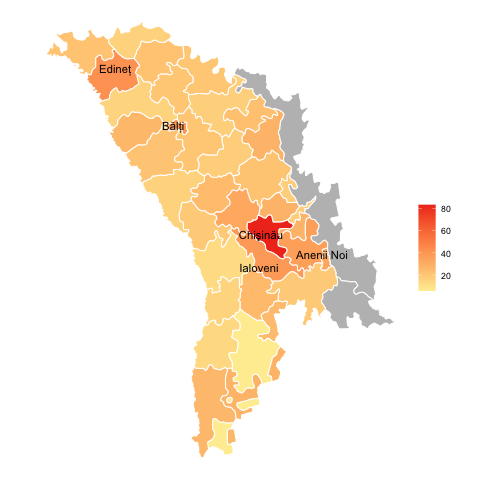
\includegraphics[width=\textwidth]{fig1.png}
\caption{Cumulative Cases of COVID-19 per thousand as of 21\textsuperscript{st} December 2021; Source - https://covid19.who.int/region/euro/country/md; Authors' own illustration}
\label{fig:map}
\end{figure}

With regards to the regulations put in place, the Republic of Moldova was under an extensive lockdown from March through mid-May (see figure~\ref{fig:timeline}). All schools were closed, as were most places of work. From mid-May, regulations were relaxed to allow recommencement of some activities as long as they allowed for adequate physical distancing of 1.5 meters. This allowed for the partial reopening of schools before the summer break though reduced class times or rotational timetables were used to ensure compliance with regulations. As of 24\textsuperscript{th} September, the distance required between individuals was reduced to 1 meter, allowing for schools to reopen more extensively and a further normalization of activities. These restrictions were in place through to the end of fieldwork.

With regards to access to modern contraceptive methods in the Republic of Moldova, existing research shows that use is far less common than in Western Europe but that socio-economic differences in contraceptive use are not identifiable \cite{janevic2012individual}. During the strictest parts of the lockdown non-emergency medical consultations were postponed which may suggest a shift away from methods requiring medical consultation towards more widely available contraceptive methods. It is very unclear however as to whether the lockdown itself has increased socio-economic inequalities in access to contraceptive methods.

\begin{figure}
\centering
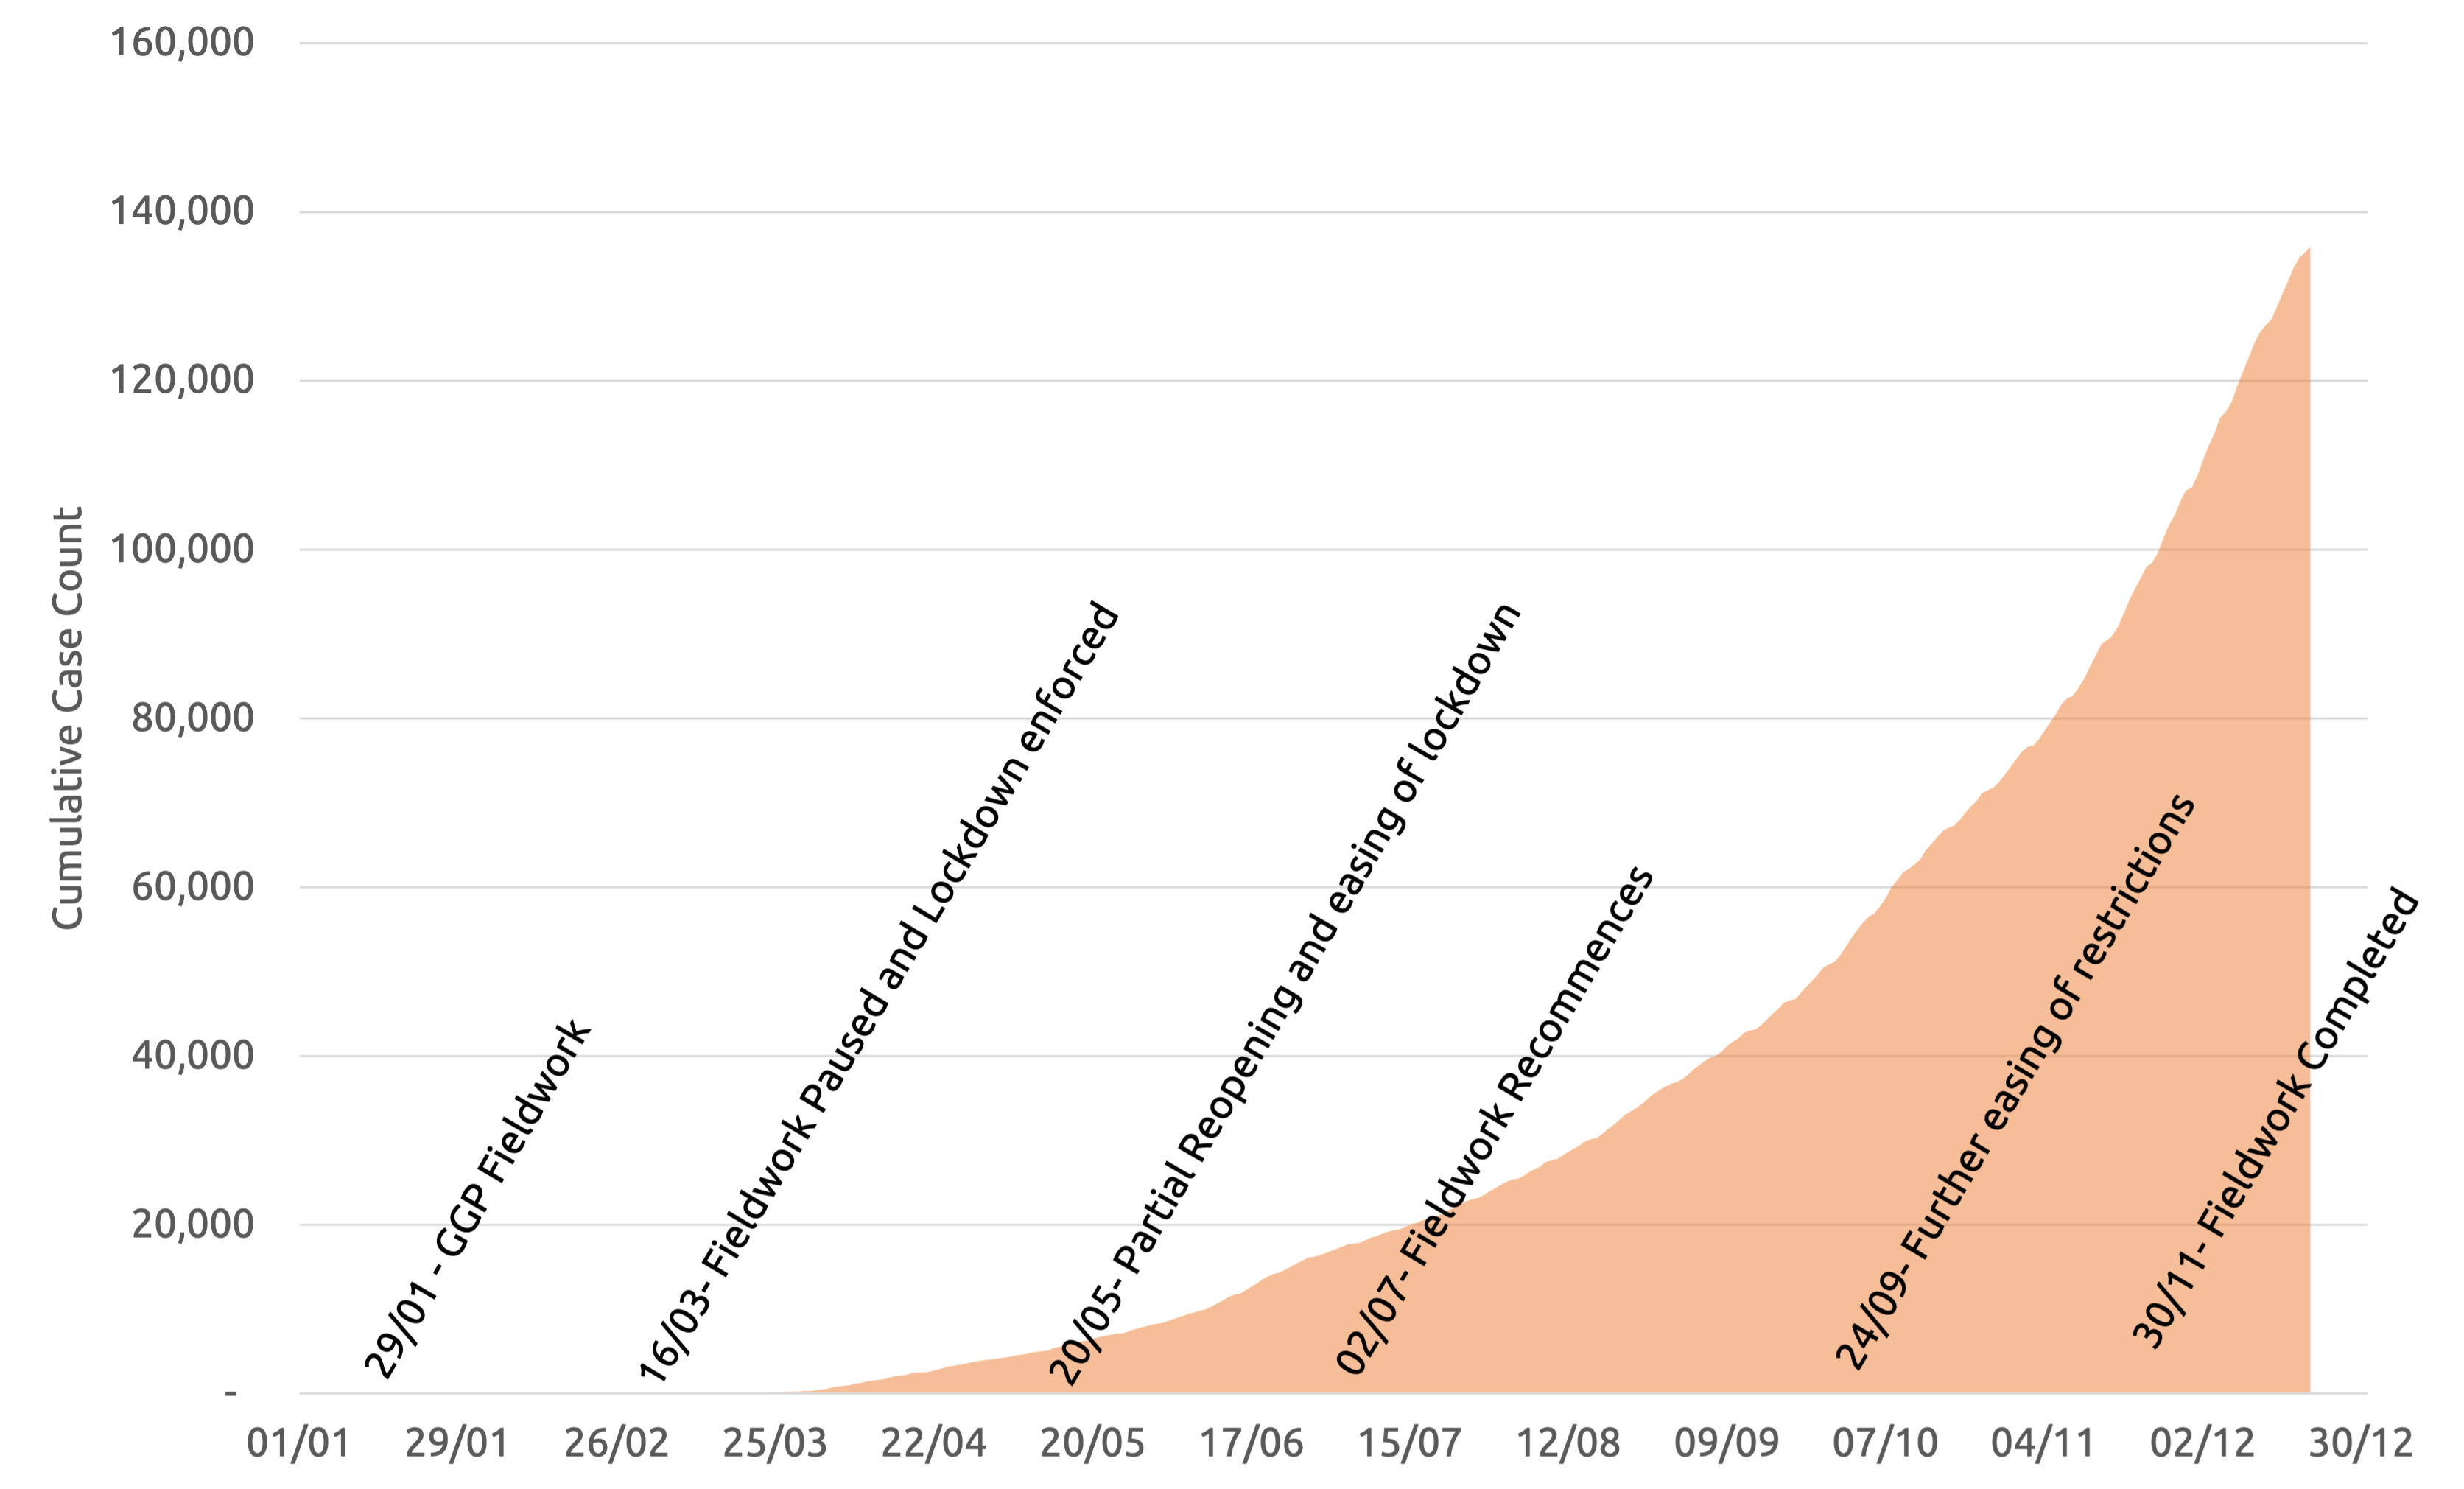
\includegraphics[width=\textwidth]{fig2.png}
\caption{Cumulative Cases of COVID-19 and timeline of events  \cite{owidcoronavirus}; 
Authors' own vizualization and annotations}
\label{fig:timeline}
\end{figure}

Travel restrictions required the quarantining of individuals arriving from other countries. This is of particular importance in the context of the Republic of Moldova given the large rates of out migration and remittances. Travel restrictions to neighbouring countries therefore represented a severe disruption to economic and family activities. 

\subsection*{Reasoned Action Approach \& Hypotheses}

To address the research question at hand, we adopt a reasoned action approach \cite{fishbein2011predicting} to study changes in capacities, intentions and behaviour over the course of the pandemic. The reasoned action approach argues that intentions and behaviour are shaped by individuals perceived behavioural control. These intentions then shape behaviour and this is moderated by the barriers and facilitators of the planned behaviour. This approach is particularly useful in this context as it clearly delineates between shifting perceptions of the individual and external exogenous influences on behaviour. This helps address the question of whether the primary influences of the pandemic on fertility are associated with its impact on the perceptions of individuals or concentrated on the practical and logistical constraints that the pandemic imposes on individuals.  This is a crucial distinction as recent research has shown that perceived barriers and uncertainty can have a significant impact on behaviour, irrespective of whether the barrier is actually realized \cite{vignoli2020reflection}. For these reasons the approach has been valuable and widely used in the fertility literature and was the basis for the design of the Generations and Gender Survey \cite{gauthier2018generations}.

By applying the reasoned action approach to data on the Republic of Moldova over the onset of the pandemic in 2020, this paper aims to not only estimate the change in intentions and behaviour brought about by the pandemic but also the degree to which these changes are associated with a shift in norms, perceived behavioural control or actual behavioural control. In doing so it will provide empirical insights to the puzzle presented by Aassve et al. (2020) regarding the impact of the pandemic on middle income countries such as the Republic of Moldova.

Based on existing empirical findings, the reasoned action approach, and the specific Moldovan context we derive the following hypotheses with regards to changes in fertility intentions and behaviour over the course of the pandemic:

\emph{H1: Sexual Activity will be lower after the onset of the pandemic than before.}
Existing research on mental well being and sexual relations during the pandemic has tended to show a decline in sexual activity during the pandemic, although these have not been as well studied in middle income countries \cite{jacob2020covid}.
\\
\emph{H2: Contraceptive use will be lower after the onset of the pandemic}\\
Existing research and theories regarding the impact of the pandemic have generally suggested that access to contraception will decline but that this decline will be acutest for those methods which require family planning services, at least at the initial stage of starting a contraception plan \cite{lindberg2020early}. 
\\
\emph{H3: The decrease in the use of contraceptives will be greatest in rural areas}\\
One of the key distinctions made by Aassve et al. (2020) in their prediction of the fertility impact of COVID is between rural and urban areas and this relates in part to the potential differential impact on access to family planning services in rural areas during the pandemic. 
\\
\emph{H4: Respondents will be less likely to be actively trying to get pregnant after the onset of the pandemic than before.}\\
In addition to a drop in sexual activity and access to family planning services, it is also expected that there will be a decline in the proportion of couples who are actively trying to conceive. This is likely due to economic uncertainty and potential wider mental health impacts. 
\\
\emph{H5: Fertility intentions will be lower after the onset of the pandemic than before.}\\
Finally, it is expected that due to the aforementioned shifts in access to family planning services, changes in sexual activity as well as negative impacts of economic uncertainty, the fertility intentions in the Republic of Moldova to fall.
\\
\emph{H6: Fertility intentions will decline most amongst households who have lost income due to the pandemic.}\\
In addition to a differential impact through access to contraception, existing research on exogenous shocks and fertility have demonstrated that households whose income is directly hit by the shock exhibit the biggest drops in fertility intentions and this has been supported by existing evidence on the impact of COVID-19 \cite{vignoli2020reflection}. We build upon this research by estimating the effect of personal loss of income due to the pandemic on fertility intentions. In addition, we examine whether low socio-economic status in and of itself can explain differences in intentions.

\section*{Data \& Methods} \label{sec:data}
\subsection*{Data}
\hl{This paper uses data from GGS Wave 1 (DOIs: 10.17026/dans-z5z-xn8g), see Gauthier, A. H. et al. (2018) or visit the GGP website (https://www.ggp-i.org/) for methodological details}. The GGS is cross-national longitudinal survey of family and relationship dynamics that is currently undertaking a new round of data collection. The questionnaire was designed by an international team of demographers through the Generations and Gender Progamme (GGP) \cite{vikat2007generations}. This questionnaire was then translated into Romanian and Russian and validated by the UNFPA and GGP.In the Republic of Moldova the fieldwork was overseen by the UNFPA in coordination with the National Bureau of Statistics of the Republic of Moldova. \hl{Informed oral consent was attained from all participants in compliance with local statistical regulations and the General Data Protection Regulation (Regulation (EU) 2016/679)}. The target sample was the residential population aged 15-79. All interviews were conducted as face-to-face. Around 15\% of the area and population of the Republic of Moldova are made up of a break away region called Transnistria which is defacto independent of the state. This regions was not covered in the data collection.  

Fieldwork commenced on the 29\textsuperscript{th} January 2020. On the 16\textsuperscript{th} March fieldwork was paused indefinitely due to physical distancing measures put in place across the Republic of Moldova. Fieldwork recommenced on the 2\textsuperscript{nd} July and was then conducted continuously until 30\textsuperscript{th} November 2020.  This resulted in 10,044 interviews. In the context of the actual prevalence of the disease, the study covers a period in which the number of cases were increasing.  3,055 interviews were conducted before the onset of the pandemic and a further 6,989 interviews were conducted afterwards. More information about the fieldwork procedures can be found on the GGP website and accompanying documentation (https://www.ggp-i.org/data/methodology/) \hl{and further information on the Moldovan fieldwork can be found on the Online Data Browser (https://www.ggp-i.org/data/browse-the-data/)}.

The overall response rate was 62.9\%. Response rates in Chișinău were much lower than the rest of the country at 41.6\% reflecting a trend that is well known for surveys in Eastern Europe \cite{fokkema2016generations}. This was despite extensive measures being undertaken to improve the response rate in Chișinău. The overall item non-response rate was very low at 3.9\% and even lower in the fertility section at 0.66\% which includes several highly sensitive questions, many of which are used in this analysis.

After the survey was interrupted due to COVID, the UNFPA and Moldovan National team requested that several items be added to measure the subjective experience of the pandemic and whether respondents felt that the pandemic had negatively affected various aspects of their lives. These questions were placed at the end of the interview to avoid effecting the core questionnaire.

\subsection*{Variables}
The hypotheses set out above refer to four separate dependent variables. Sexual activity is measured using question FER13 \footnote{Did you have sexual intercourse in the past 4 weeks? Yes or No}. Contraceptive usage is measured using FER12 \footnote{Are you or your partner using or doing any of these things to prevent pregnancy at this time? Please name all of the things you use or do. Condom, Pills, IUD, Diaphragm, Foam/Cream/Jelly/Suppository, Injectables, Implants, Pesona, Morning after pill, Withdrawal, safe period method, vaginal ring, female condom.} Those who selected a modern contraceptive method (Condom, Pills, IUD, Diaphragm, Foam/Cream/Jelly/Suppository, Injectables, Implants, Morning after pill, vaginal ring, female condom) were coded as 1 to reflect contraceptive usage (CU) and those who didn't were coded as 0. To measure whether a couple is actively trying to get pregnant FER10a was used \footnote{Are you or your current partner trying to get pregnant? Yes or No"}. The dependent variables are presented in table 1.
\begin{center}
\begin{table}[htbp]\centering
\def\sym#1{\ifmmode^{#1}\else\(^{#1}\)\fi}
\caption{Dependent Variables}
\begin{tabular}{l*{2}{cc}}
\hline\hline
                    &\multicolumn{1}{c}{(1)}&            &\multicolumn{1}{c}{(2)}&            \\
                    &Pre Lockdown&            &Post Lockdown&            \\
                    &        mean&          sd&        mean&          sd\\
\hline
Had intercourse     &       0.852&       0.356&       0.886&       0.318\\
Contraceptive Use   &       0.389&       0.488&       0.408&       0.492\\
Trying to Conceive  &       0.087&       0.282&       0.059&       0.235\\
Fertility Intention &       0.331&       0.471&       0.350&       0.477\\
\hline
Observations        &         734&            &        1909&            \\
\hline\hline
\end{tabular}
\end{table}

\end{center}
To measure a respondents fertility intention FER14 was used \footnote{Do you intend to have a/another child during the next three years? Please take into account only biological children. Definitely yes, probably yes, unsure, probably no, definitely no."}. It should be noted that the questions are only asked to women aged 18-49 and men who have a female partner aged 15-49. If the respondent or their partner were pregnant at the time of the interview were also excluded from the analysis. If they were not sure yet, they were included in the analysis. Those without a co-resident partner were asked these questions but we restricted the analysis to those with a partner and aged 18-40 in order to focus the analysis on those individuals most likely to have medium term fertility intentions.
\begin{center}
\begin{table}[htbp]\centering
\def\sym#1{\ifmmode^{#1}\else\(^{#1}\)\fi}
\caption{Independent Variables}
\begin{tabular}{l*{2}{cc}}
\hline\hline
                    &\multicolumn{1}{c}{(1)}&            &\multicolumn{1}{c}{(2)}&            \\
                    &Pre Lockdown&            &Post Lockdown&            \\
                    &        mean&          sd&        mean&          sd\\
\hline
Age                 &      36.413&       7.677&      35.819&       7.618\\
Sex of Respondent [Ref = Female]&       0.357&       0.479&       0.327&       0.469\\
Education Level     &       0.000&       0.000&       0.000&       0.000\\
Employment Status   &       0.658&       0.475&       0.654&       0.476\\
Number of Coresident Children&       1.598&       1.145&       1.553&       1.044\\
Urban Resident      &       0.475&       0.500&       0.335&       0.472\\
Willingness to answer&       0.655&       0.476&       0.653&       0.476\\
\hline
Observations        &         734&            &        1909&            \\
\hline\hline
\end{tabular}
\end{table}

\end{center}
Independent variables of interest that are used in the analysis are age, sex, educational level\footnote{measured as whether an individual has tertiary qualifications or not}, employment status\footnote{whether someone is in paid employment or on leave from paid employment}, region, whether they live in an urban or rural area, and whether they have co-resident children (see table 2). Questions on the impact of the pandemic on household income were only asked to the sample interviewed after the onset of the pandemic. For this analysis, those who responded that there was a large or very large impact on their household income were coded as 1 and the rest, including those who were interviewed before the onset of the pandemic, were coded as 0. The summary all the variables used can be found below:
\begin{figure}
\centering
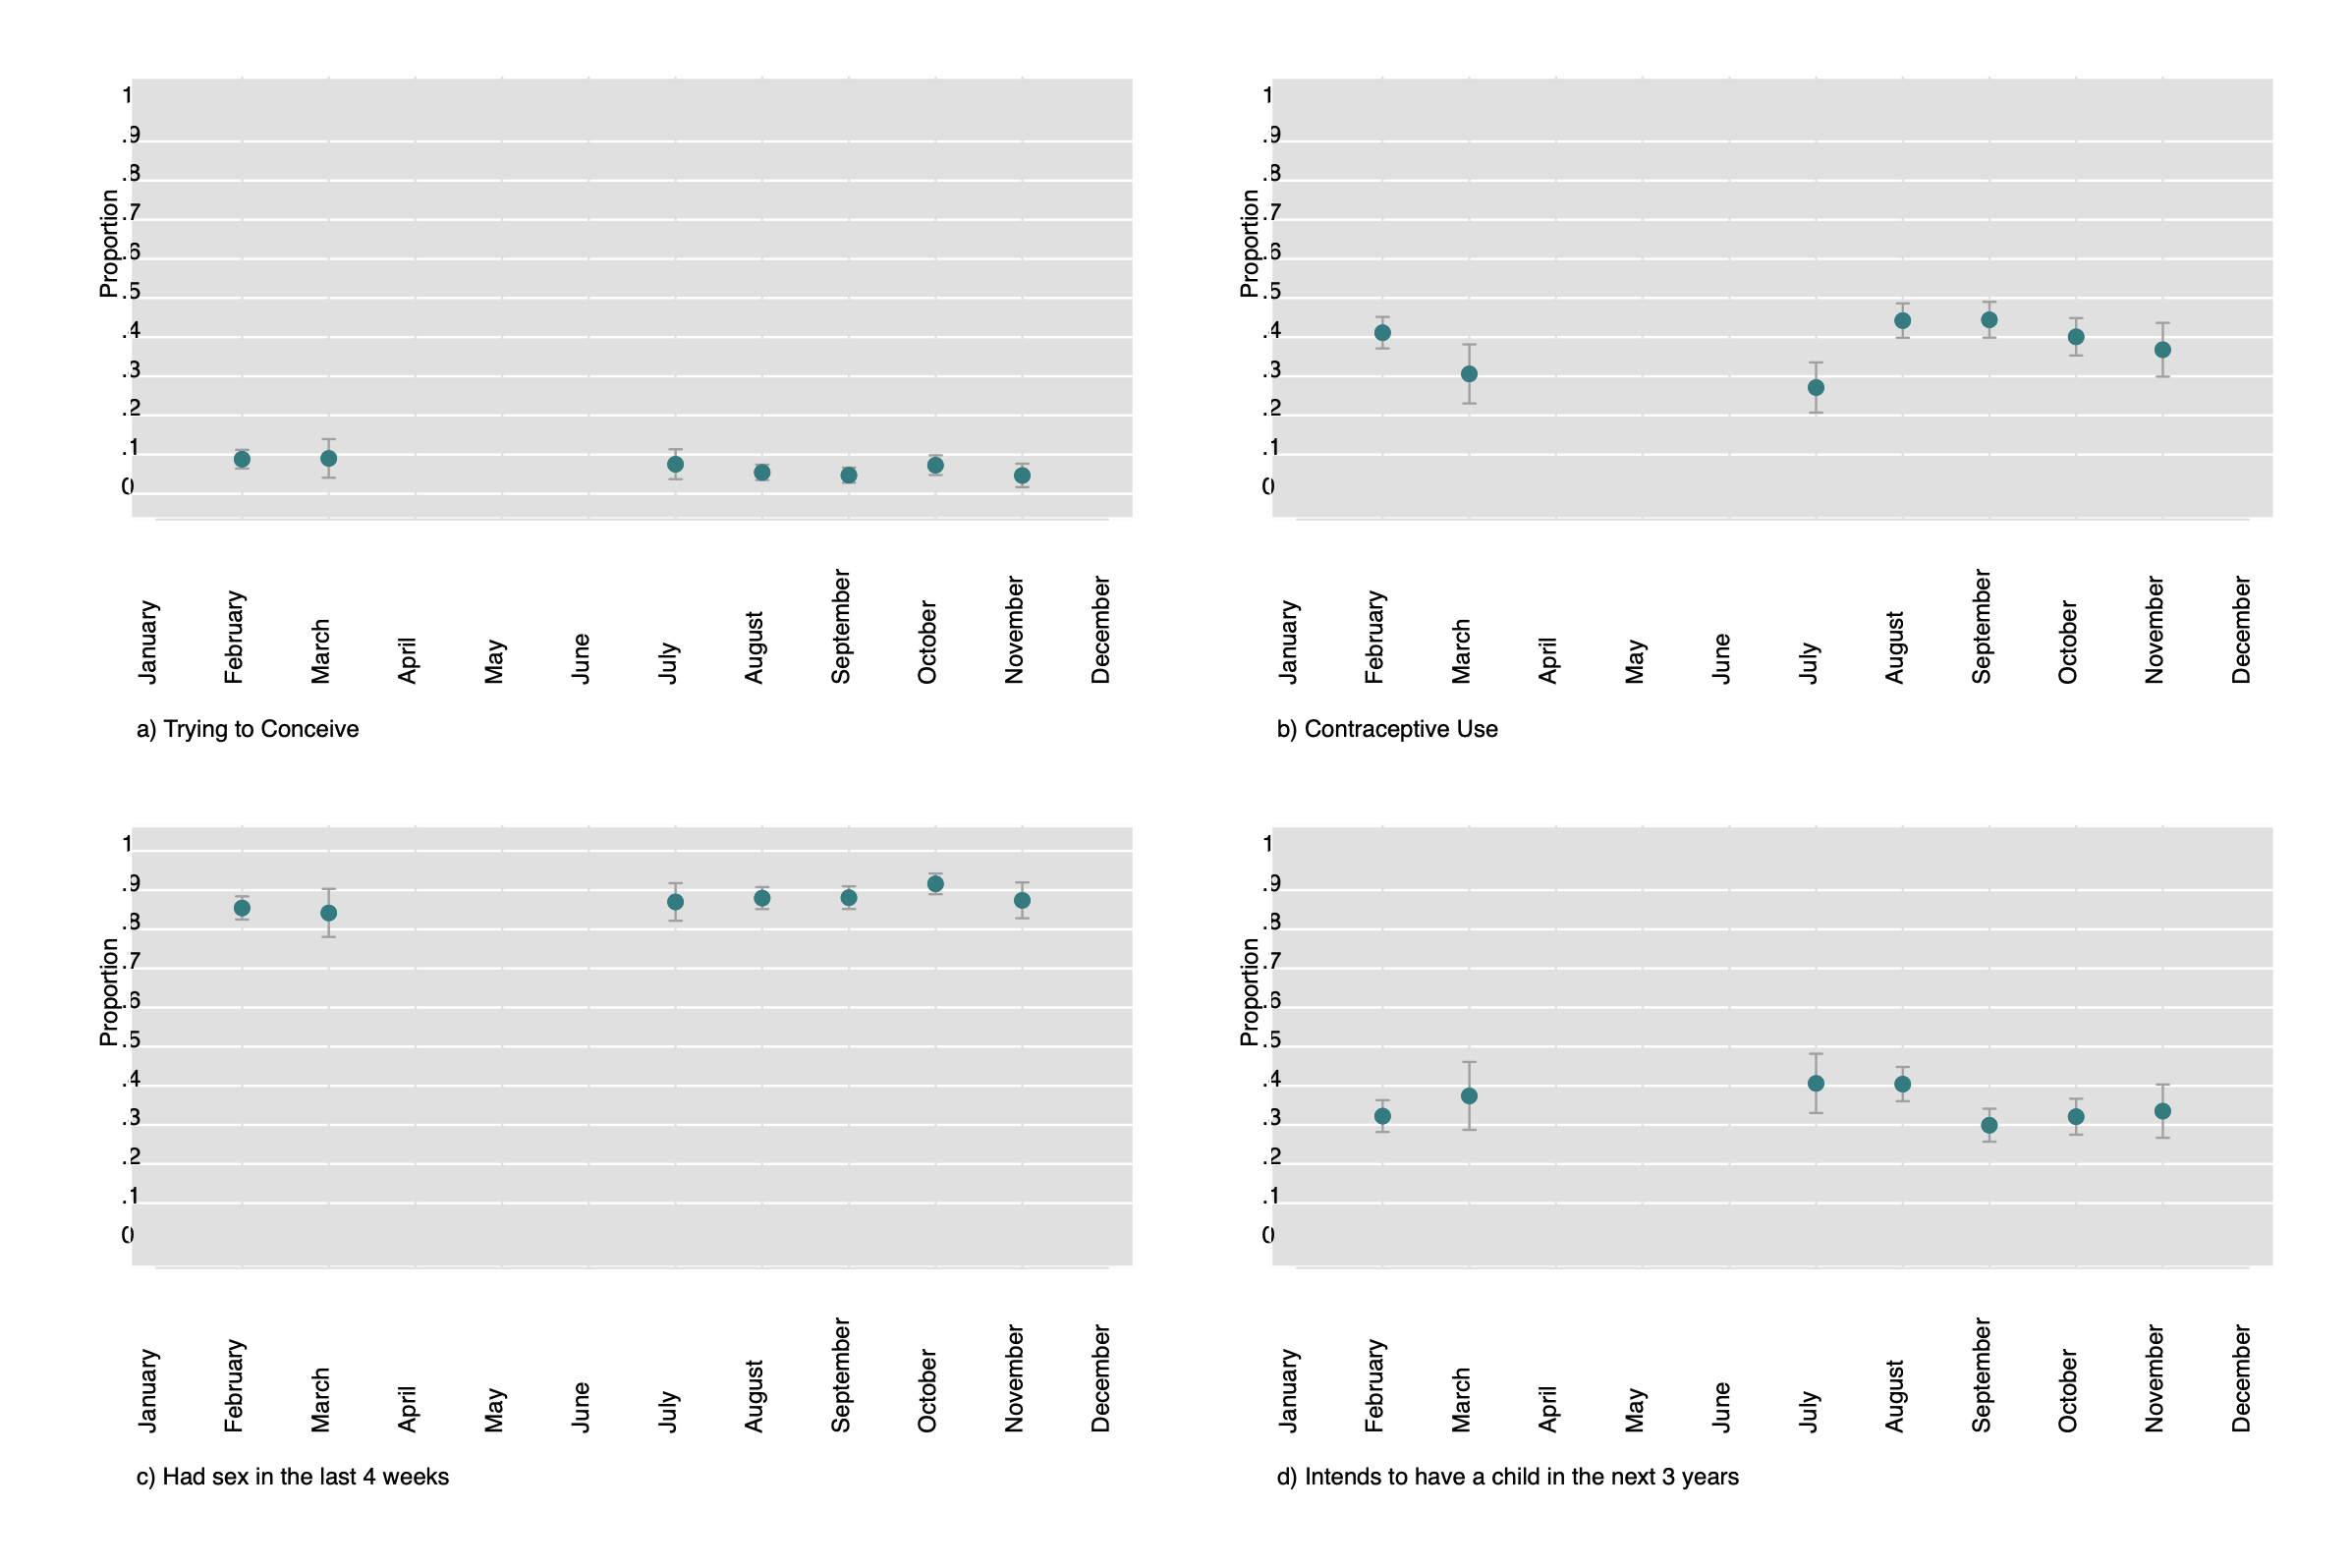
\includegraphics[width=\textwidth]{fig3.png}
\caption{\hl{Proportion of 18-49 year old's that are currently trying to conceive, using modern contraceptive methods, that have had sex in the last four weeks and that have fertility intentions in the next 3 years}}
\label{fig:deps_month}
\end{figure}
\subsection*{Analytic Strategy}
For the analysis, the hypotheses are tested in turn using a logit model, using a dichotomous variable to represent the period before and after the onset of the pandemic. However, the onset of the pandemic has itself been made up of several stages in the Republic of Moldova. To test the findings in these models, they were also run with time specified as a categorical month variable to allow for variation in the impact of the pandemic over time. Generally, the effects were stable over the months preceding the resumption of fieldwork and so the simpler pre and post measure is used but where monthly variations are statistically significant, they are reported. 

Post stratification weights were applied based on age, gender and region of residence. The primary internal validity concern relates to the progression of fieldwork in the Republic of Moldova and its association with the progression of the pandemic. In survey research it is common to observe that specific groups respond earlier in the fieldwork period than others. It is likely that these different groups will have different fertility intentions and behaviours and this thus threatens to bias the estimates. It is likely that those which are hardest to reach are those more likely to migrate or be less settled and these are also those individuals least likely to be intending to have children. However, the fieldwork in the Republic of Moldova was structured such that various districts of the sample were exploited at different times and were exhausted before the fieldwork team moved on to the next district. The onset of the pandemic coincided with the completion of the first round of districts which may go someway to mitigating this effect. The districts examined in each round of fieldwork were approximately representative of the country as a whole.

However, to further test against this potential bias, models were run which including variables indicating respondent willingness to participate and the number of others present during the interview. \hl{These variables are recorded at the end of the interview by interviewers and are not seen by respondents. The willingness to answer questions is a standard quality control item in the GGS and is marked on a scale of 1-10}. Physical distancing measures meant that some interviews were conducted outdoors or in larger rooms and there was therefore potentially less privacy in fieldwork after the onset of the pandemic, leading to increased social desirability bias. 

Whilst these variables did exhibit a correlation with fertility behaviours and intentions, their inclusion in the models didn't not change the significance or direction of the coefficients reported here. \hl{There was no statically significant difference in 'willingness to answer questions' pre and post pandemic (see table 2) and this was also true of other data quality measures such as item non-response, length of interview and interview interruptions}. \hl{The migration characteristics of respondents and their partners in the pre and post lockdown populations were also compared and no statistically significant differences were found, suggesting that there was not increased inward or outward migration associated with the lockdown which could account for differences in fertility behaviours}.
\newpage

\section*{Results} \label{sec:result}
\begin{table}[htbp]\centering
\def\sym#1{\ifmmode^{#1}\else\(^{#1}\)\fi}
\caption{Results of logistic regression on pre \& post population [Log Odds]}
\begin{tabular}{l*{6}{c}}
\hline\hline
                    &\multicolumn{1}{c}{(1)}&\multicolumn{1}{c}{(2)}&\multicolumn{1}{c}{(3)}&\multicolumn{1}{c}{(4)}&\multicolumn{1}{c}{(5)}&\multicolumn{1}{c}{(6)}\\
                    &\multicolumn{1}{c}{Had sex}&\multicolumn{1}{c}{CU}&\multicolumn{1}{c}{CU}&\multicolumn{1}{c}{Trying}&\multicolumn{1}{c}{Intention}&\multicolumn{1}{c}{Intention}\\
\hline
main                &                     &                     &                     &                     &                     &                     \\
Post Lockdown       &       0.326\sym{**} &       0.138         &      0.0515         &      -0.608\sym{***}&     0.00208         &     -0.0359         \\
                    &      (2.58)         &      (1.66)         &      (0.46)         &     (-3.98)         &      (0.02)         &     (-0.32)         \\
[1em]
Age                 &     -0.0129         &     -0.0240\sym{***}&     -0.0237\sym{***}&     -0.0267\sym{**} &      -0.117\sym{***}&      -0.117\sym{***}\\
                    &     (-1.65)         &     (-4.77)         &     (-4.72)         &     (-2.91)         &    (-18.53)         &    (-18.54)         \\
[1em]
Male                &       1.175\sym{***}&      -0.218\sym{**} &      -0.215\sym{**} &      0.0985         &       0.714\sym{***}&       0.715\sym{***}\\
                    &      (8.83)         &     (-2.90)         &     (-2.85)         &      (0.68)         &      (8.24)         &      (8.25)         \\
[1em]
Number of Coresident Children&     -0.0799         &      0.0421         &      0.0431         &      -0.674\sym{***}&      -0.572\sym{***}&      -0.573\sym{***}\\
                    &     (-1.53)         &      (1.18)         &      (1.21)         &     (-8.48)         &    (-12.59)         &    (-12.60)         \\
[1em]
Higher Education    &       0.241         &       0.382\sym{***}&       0.376\sym{***}&     -0.0467         &     -0.0204         &     -0.0213         \\
                    &      (1.77)         &      (4.58)         &      (4.49)         &     (-0.29)         &     (-0.21)         &     (-0.22)         \\
[1em]
Working             &       0.385\sym{**} &       0.187\sym{*}  &       0.185\sym{*}  &       0.103         &     -0.0222         &     -0.0180         \\
                    &      (3.21)         &      (2.27)         &      (2.25)         &      (0.64)         &     (-0.24)         &     (-0.19)         \\
[1em]
Urban               &       0.164         &      0.0316         &     -0.0994         &      0.0231         &       0.272\sym{**} &       0.270\sym{**} \\
                    &      (1.23)         &      (0.38)         &     (-0.71)         &      (0.15)         &      (2.87)         &      (2.85)         \\
[1em]
1                   &      0.0591         &      -0.407\sym{***}&      -0.411\sym{***}&       0.203         &     0.00303         &     0.00806         \\
                    &      (0.49)         &     (-5.26)         &     (-5.30)         &      (1.29)         &      (0.03)         &      (0.09)         \\
[1em]
Others Present      &      0.0783         &       0.377\sym{***}&       0.377\sym{***}&      -0.350         &     -0.0770         &     -0.0762         \\
                    &      (0.48)         &      (3.81)         &      (3.82)         &     (-1.59)         &     (-0.67)         &     (-0.67)         \\
[1em]
Post Lockdown X Urban&                     &                     &       0.194         &                     &                     &                     \\
                    &                     &                     &      (1.16)         &                     &                     &                     \\
[1em]
Drop in Income=1    &                     &                     &                     &                     &                     &      0.0661         \\
                    &                     &                     &                     &                     &                     &      (0.66)         \\
[1em]
Post Lockdown X Drop in Income=1&                     &                     &                     &                     &                     &           0         \\
                    &                     &                     &                     &                     &                     &         (.)         \\
[1em]
Constant            &       1.611\sym{***}&       0.263         &       0.323         &      -0.597         &       3.979\sym{***}&       3.978\sym{***}\\
                    &      (4.70)         &      (1.19)         &      (1.42)         &     (-1.48)         &     (15.01)         &     (15.01)         \\
\hline
Observations        &        2289         &        2230         &        2230         &        2220         &        2114         &        2114         \\
\hline\hline
\multicolumn{7}{l}{\footnotesize \textit{t} statistics in parentheses}\\
\multicolumn{7}{l}{\footnotesize \sym{*} \(p<0.05\), \sym{**} \(p<0.01\), \sym{***} \(p<0.001\)}\\
\end{tabular}
\end{table}

The first set of results are presented in table 3. Model 1 indicates that respondents after the lockdown were 38\%\footnote{$exp(0.324) = 1.38$} more likely to report having had sex than respondents prior to lockdown and this is significant at $p < 0.05$. This runs counter to the first hypotheses and suggests that there has in fact been a small increase in sexual activity after lockdown. When looking at the basic descriptive statistics by gender, the difference between pre and post lockdown is larger amongst women (82\% v 86\%) than men (92\% v 94\%). 
The second model indicates that the \hl{odds of using contraceptives} were 40\%\footnote{\hl{$1 - exp(-0.517) = 0.404$}} lower after the lockdown. This is a large downturn and is inline with the second hypothesis and the assertion by Aassve et al. (2020) that contraceptive usage would be constrained. The third model tested whether there was a difference in the impact of the lockdown between urban and rural areas. \hl{The coefficient for lockdown} was positive and significant suggesting that the impact on access was indeed lesser in urban areas (see figure~\ref{fig:marginal}). \hl{In further analysis (not shown), interaction terms were also included between education level and the impact of lockdown and no significant effects or improvement in model fit were found. This suggests that the fall in contraceptive usage was geo-spatially orientated rather than a reflection of an educational gradient}.

The fourth model shows that respondents were \hl{41\%}\footnote{\hl{$1 - exp(-0.532) = 0.587$}} less likely to be trying to conceive post lockdown than prior, dropping from 8.7\% to 5.7\%. That is a large drop off in those actively trying to conceive and it supports the fourth hypothesis. The fifth and sixth models revealed no differences in the medium term fertility intentions of respondents between pre and post lockdown and there was no difference identified between those who were financially impacted by the lockdown and those who weren't. 

\begin{figure}
\centering
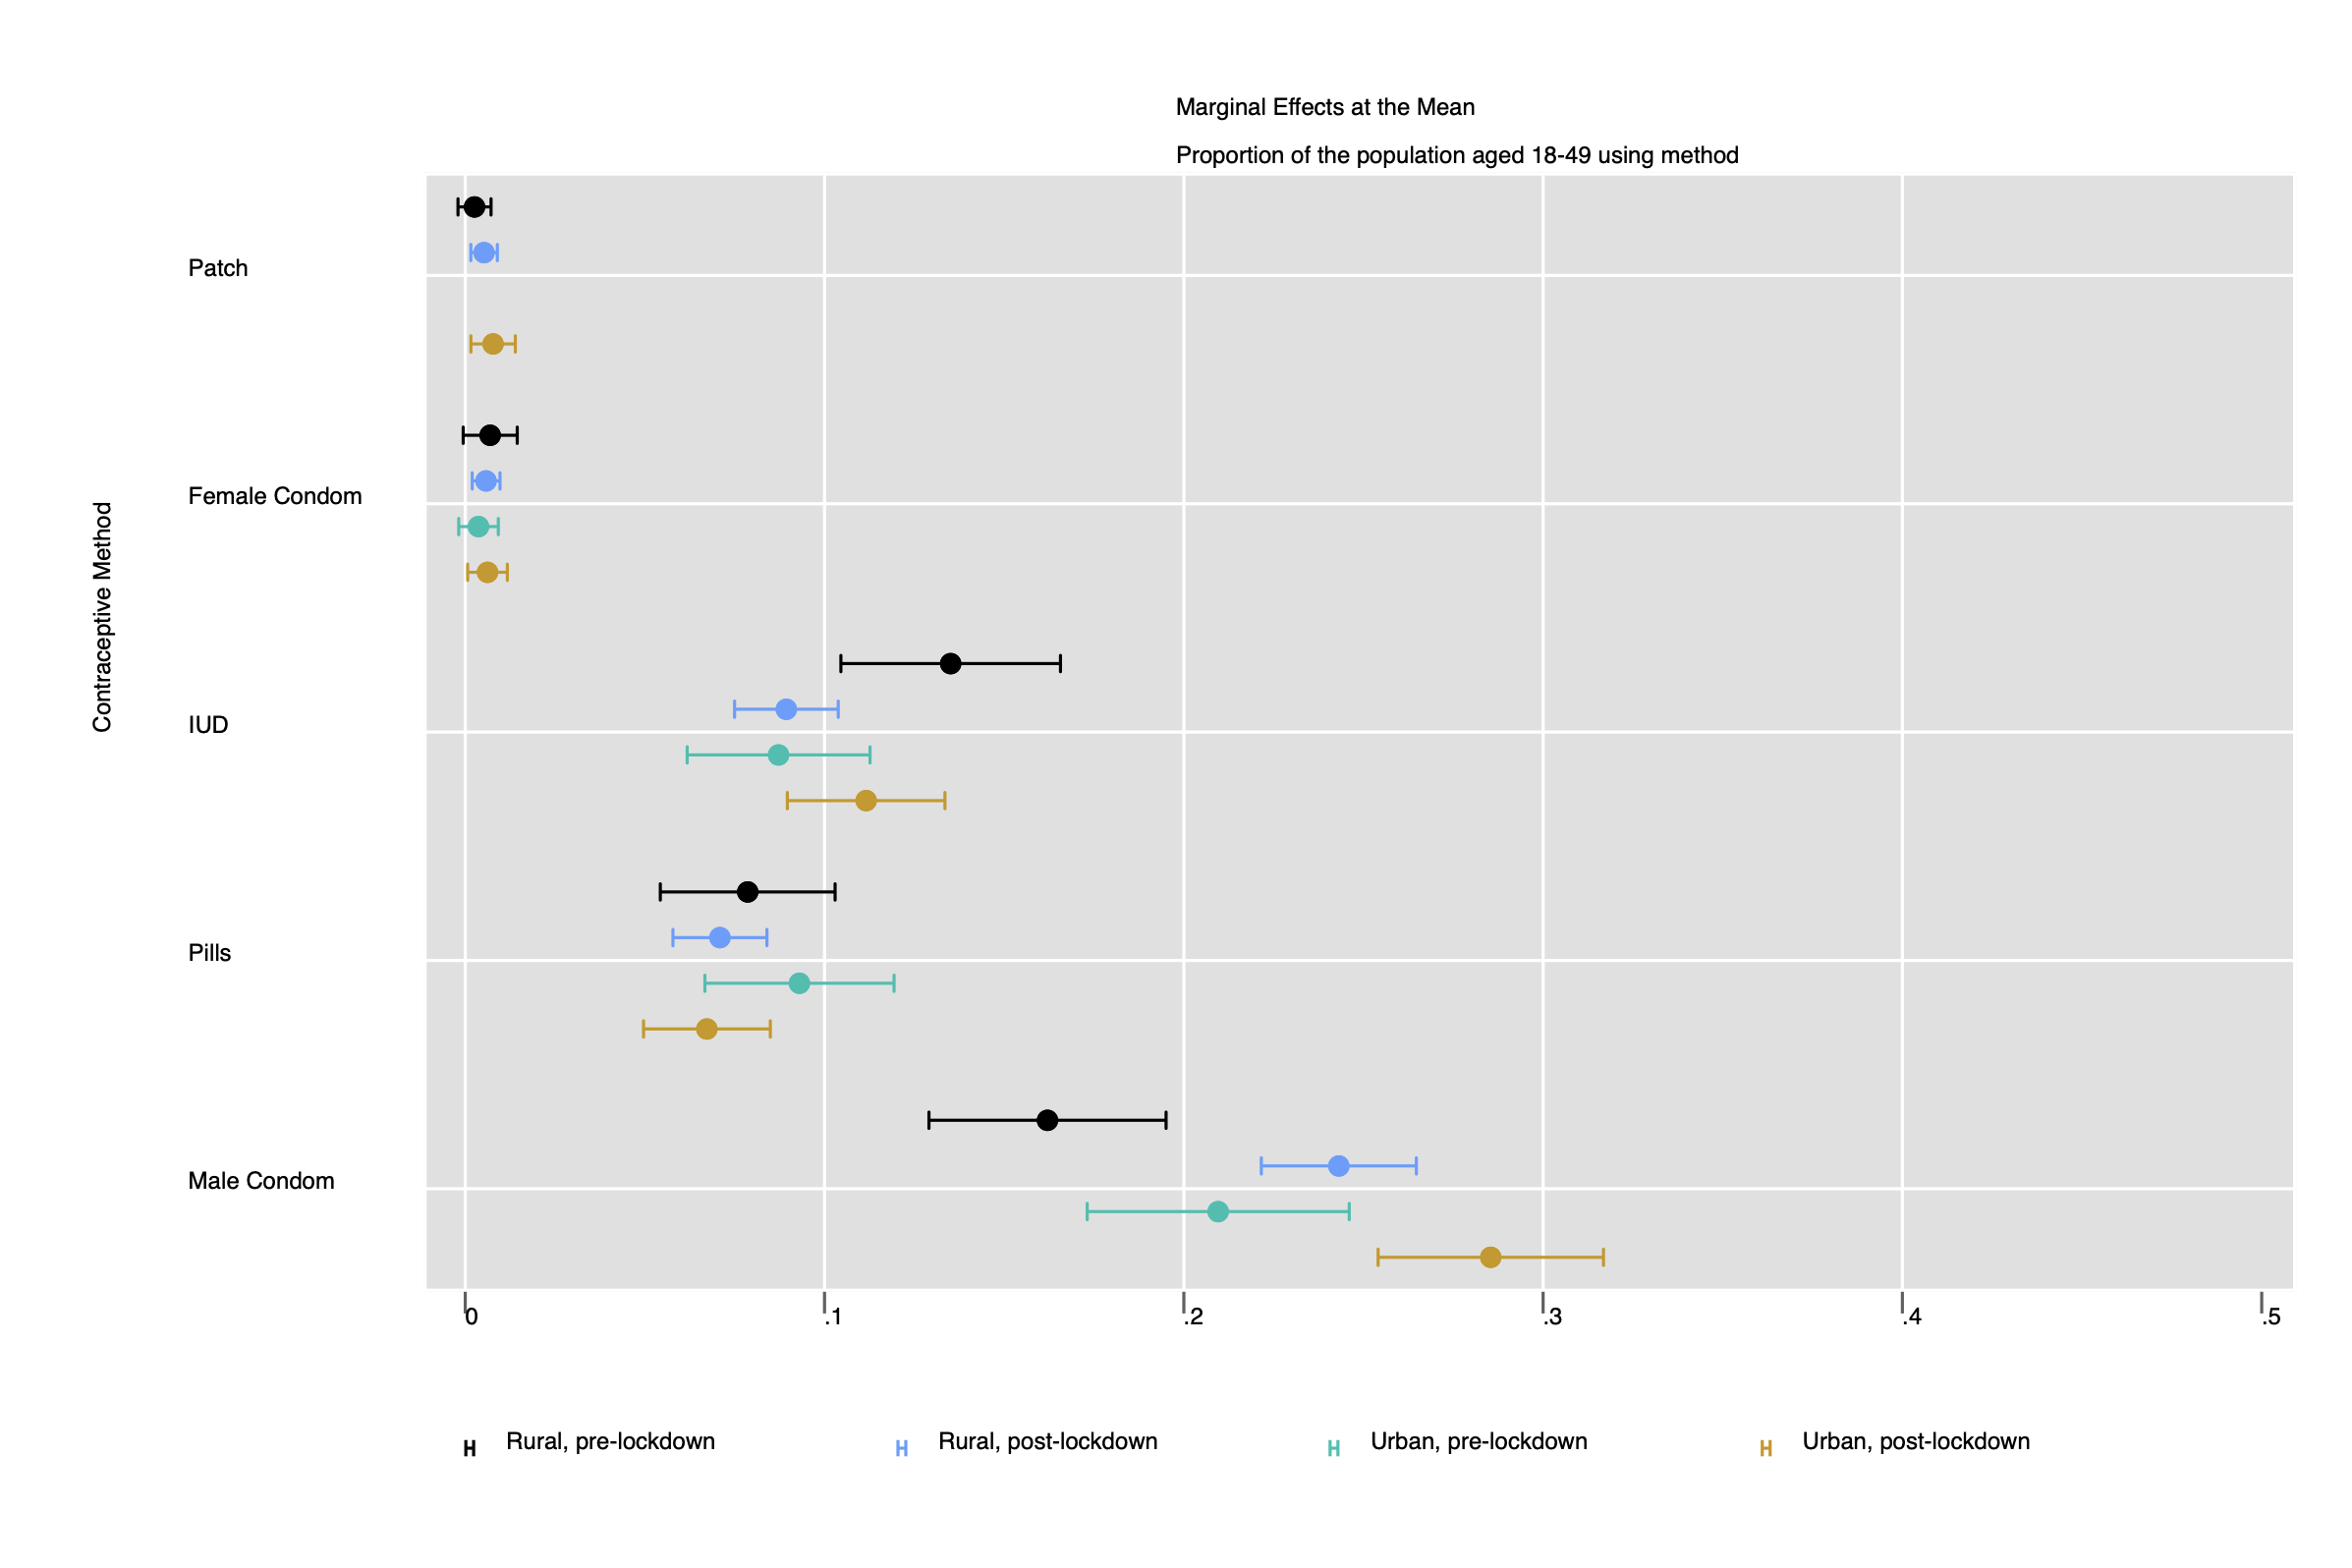
\includegraphics[width=\textwidth]{fig4.png}
\caption{\hl{Estimated probabilities of contraceptive use pre and post lockdown}}
\label{fig:marginal}
\end{figure}

In terms of the robustness of the results, the potentially confounding factors are associated with the fieldwork process itself. Respondents in the second part of the fieldwork may have been more reluctant respondents. We do note that the perceived willingness to answer questions was associated with lower levels of contraceptive use, \hl{which is to be expected from a non-cooperative respondent as they may want to avoid providing details of a specific contraceptive method. This is unlikely to explain the observed effect of lockdown on contraceptive usage however, as the difference in means between pre and post lockdown is small, statistically insignificant and in the opposite direction from that of the effect of lockdown on contraceptive usage (see table 2). To ensure that a differential in 'willingness to answer' was not driving this effect an interaction effect was included with the lockdown variable but the cofficient was not significant (results not shown).}

We also considered the role of others being present during an interview. This was included because there was a change in fieldwork protocols after lockdown which may have influenced responses as it was harder to hold interviews alone. This was also only apparent for contraceptive usage in models 2 and 3 but interestingly, those with others present reported higher levels of contraceptive usage which is contrary to expectations. \hl{It was expected that people would be shy about declaring specific contraceptive methods but the results suggest that the social desirability bias may operate the other way, with respondents more likely to declare a contraceptive method if others are present. This could suggest that the drop in contraceptive usage after lockdown is larger than reported.}

The results of the analysis indicate large shifts in aggregate short term fertility behaviour, whilst medium term intentions remain constant. What remains to be understood is whether the decrease in contraceptive use in particular is largest amongst those who have medium term fertility intentions or whether it is a decrease amongst those who don't. In the terms of the United Nations definition of Sustainable Development Indicator 3.7.1, this is distinction between an unmet family planning needed associated with limiting or spacing of children. 

Amongst those with medium term fertility intentions, usage of contraception 24.8\% from 62\% pre lockdown to 45\%. Amongst those without any medium term fertility intentions, it fell by \hl{26\%} from 66\% to 50\%. This is a large decrease in both groups which suggests that there are substantial increases in the unmet needs with regards to both limiting and spacing of children.  

\newpage
\section*{Conclusion}\label{sec:conclusion}

This paper seeks to understand the impact of the COVID-19 Pandemic and associated social measures on fertility behaviour in the Republic of Moldova. 75\% of the world's population live in middle income countries such as the Republic of Moldova according to the world bank, and as laid out by Aassve et al., the potential impact of the pandemic on fertility behaviour in these countries is hard to anticipate. This paper offers some insights into the complex impact the pandemic has had on fertility behaviour but ultimately reinforces the assertion made by Aasvve et al. that the long term demographic impact is hard to ascertain. 

In terms of the overall impact on fertility there are several notable findings from this paper. Firstly, we observe a dramatic fall in the proportion of respondents trying to conceive of around 41\%. If this was reflected in a similar fall in the birth rate the demographic consequences would be considerable. However, the medium term fertility intentions do hold steady in our analysis, suggesting that there might be a delay in births rather than a permanent decline in the birth rate. The extent to which this is true is unknown and will only become evident as the impact of the pandemic both in terms of its public health impact but also its wider social and economic impact become apparent. This paper can not reflect on whether these deferred conceptions will be realized because that is simply not knowable yet but existing research indicates that there is strong association between short term fertility intentions and behaviour \cite{dommermuth2015realization}. 

The other factor that Aassve et al. point to which complicates the picture in middle income countries, is the access to family planning services. There was a considerable decrease of around 40\% in contraceptive usage during the pandemic, amongst those couples with and without medium term fertility intentions. Some existing literature has suggested that this would be offset by a fall in sexual activity associated with the socio-economic impact of the pandemic but this was not observed. This greatly increases the risk of unplanned pregnancies and births and the consequences that has for both the parents and child. It could well be that the unplanned births offset the fall in conception efforts amongst those with medium term fertility intentions, which is the question that Aassve raises. 

However the micro-level analysis presented here illustrates that this point is in many ways only secondary. The more pressing and long term issue is the potential increase in unplanned pregnancies and regression in active control that individuals have over their family planning. The consequence of the pandemic on fertility in middle income countries could therefore be an increase in births amongst those who were not planning on having children and a decrease in births amongst those who were. 

There are several limitations we can point to in this paper. Most importantly, the analysis is effectively a repeated cross-sectional study. The differences we observe are between and not within individuals. A longitudinal study would offer far greater insights into the shifts in fertility behaviour and the underlying dynamics. Unfortunately this was not possible with the data at hand. There are longitudinal panels which offer such data in high income countries (For example see \cite{luppi2020impact}). We are unaware of any such longitudinal data for middle income countries however and the impact of the pandemic on fertility in such a context was the main focus of this paper. \hl{This will be particularly important when considering the medium and long term impacts of the pandemic as it will alter all manner of social processes such as partnership formation, educational attainment, labour market trajectories and many others. Understanding the impact of these processes on fertility behaviours in the aftermath of the pandemic is vital but this analysis only considers the short term impact on fertility intentions.}

The second limitation is the focus of the analysis purely on survey data. Survey data provides subjective measures and insights into cognitive processes that are exceptionally valuable for fertility research. However, there have been serious developments in the use of new forms of data in the study of demography, such as google trends data, that could prove useful in validating the results found here \cite{alburez2019demography}\cite{wilde2020covid}. Doing so lies outside the scope of this paper given that the theoretical framework is deeply embedded within the survey data used and because the analysis of these new data forms require sufficient detail and attention that this paper can not accommodate. 

Finally, the study focuses on the Republic of Moldova as an example of a middle income country. The Republic of Moldova is however a very atypical country. Unlike most middle income countries it is in Europe and has a land border and association agreement with the European Union which have a significant gravitational impact on the economy and wider society. Whilst the Republic of Moldova does exhibit poor access to family planning in line with many middle income countries, it does not exhibit some of the crucial challenges that Aassve et al. referred to. The urban-rural divide in access to family planning in the Republic of Moldova may not be so great given that the country is relatively small in both area and population when compared with more notable middle income countries such as China, India, Indonesia or Brazil. It is the demographic impact in these larger and more populous countries that will ultimately shape the demographic consequences of the pandemic. Nevertheless, the analysis here provides insights into a middle income country when high quality data is sparse and helps elucidate some of the micro level dynamics at play in such contexts. 

This paper has provided insights into fertility behaviour at the micro level in a middle income country context that is often understudied and yet of critical importance in understanding the wider demographic implications of the pandemic. The data used has enabled us to look at multiple dimensions of fertility behaviour and how they interrelate. There is strong evidence for large short-term effects on fertility behaviour. Crucially, for those with no medium term fertility intentions there is a significant increase in unmet family planning needs and yet for those with medium term fertility intentions there is apparent deferment in actively trying to conceive. It will be vital that this is continuously studied as time passes in order to understand how short term and medium term intentions converge over time as the impact of the pandemic becomes apparent. 

\section*{Acknowledgments}
Particular thanks to the UNFPA Moldova, National Bureau of Statistics of the Republic of Moldova and the Ministry of Health, Labour and Social Protection of the Republic of Moldova for support in conducting the Gender and Generations Programme in the conduct of the study. This analysis in this paper was conducted in collaboration with the UNFPA Moldova and the Ministry of Health, Labour and Social Protection of the Republic of Moldova in response to the onset of the COVID-19 Pandemic during the fieldwork of the Moldovan GGS in 2020. Both parties reviewed and provided comments on earlier and current versions of the analysis. The contents of this publication do not necessarily reflect the views or policies of the UNFPA Moldova and the Ministry of Health, Labour and Social Protection.

\nolinenumbers

% Either type in your references using
% \begin{thebibliography}{}
% \bibitem{}
% Text
% \end{thebibliography}
%
% or
%
% Compile your BiBTeX database using our plos2015.bst
% style file and paste the contents of your .bbl file
% here. See http://journals.plos.org/plosone/s/latex for 
% step-by-step instructions.
% 
\bibliography{references}





\end{document}

